\section{Grappa Overview}

\begin{figure}[t]
\begin{center}
  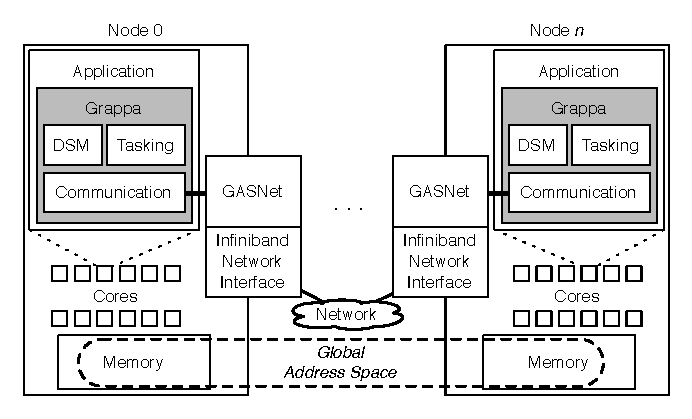
\includegraphics[width=0.95\columnwidth]{figs/system-overview}
\begin{minipage}{0.95\columnwidth}
  \caption{\label{fig:grappa} Grappa system overview}
\end{minipage}
\vspace{-3ex}
\end{center}
\end{figure}


Grappa (Figure~\ref{fig:grappa}) provides three main software components:
a \textbf{tasking system} with lightweight multithreading to tolerate
latency and workstealing to automate load balance;
a \textbf{distributed shared memory} (DSM) providing high aggregate
random access bandwidth for both normal and synchronized operations;
and a \textbf{communication layer}, which is largely invisible to the software developer but helps to improve network performance when applications read and write only small pieces of data.
In the next three sections we describe both the programmer's view of Grappa's main capabilities and how they are implemented.


